% -*-coding: utf-8 -*-

V této kapitole popíšeme několik vybraných optimalizačních algoritmů. Zdaleka nejde o průřez všemi typy algoritmů\footnote{obsáhlejší přehledy lze nalézt například v \cite[p.~23]{GO ebook}, \cite{wiki metaheur}}, ale alespoň získáme představu s čím se budeme muset při hledání obecného formalismu potýkat. Na konci zmíníme obecné principy, myšlenky a problémy, které se objevují napříč všemi algoritmy, a které bychom taktéž chtěli v našem modelu pokrýt.

\section{Základní pojmy}

\par{\textbf{Účelová funkce (fitness)} je funkce, jejíž hodnotu se algoritmus snaží optimalizovat. Optimalizaci lze vždy formulovat jako minimalizaci.}

\par{\textbf{Kandidátní řešení (jedinec)} je struktura data, z nichž je možné spočíst hodnotu účelové funkce. Manipulací s těmito daty se algoritmus snaží najít nejlepší možné řešení.}

\par{\textbf{Stavový prostor} je prostor všech jedinců.}

\par{\textbf{Populace} je soubor jedinců s nimiž algoritmus aktuálně pracuje. Ne každý algoritmus potřebuje populaci}

\par{Metaheuristika je obecný návrh algoritmu popisující myšlenky, jakými budeme jedince krok po kroku zlepšovat aniž bychom dělali složitější předpoklady o účelové funkci, charakteru problému nebo implementaci. Myšlenky obsažené v metaheuristice zřídkakdy zajišťují konvergenci algoritmu k optimálnímu řešení.}

\section{Algoritmy}

Pokud není řečeno jinak, u algoritmů vždy popisujeme jeden jejich krok a vynecháváme ukončující podmínku, kterou bývá často konvergence algoritmu, nebo dosažení dostatečně nízké fitness.

\subsection{Simulované žíhání a zrychlené simulované žíhání}

\textbf{Simulované žíhání} (SA -- Simulated Annealing) \cite{SA Hajek}, \cite{SA Tsitsiklis} je metaheuristika založená na analogii s chladnutím kovu. Při chladnutí se atomy snaží zaujmout pozici s co nejnižší energií; když je teplota vysoká, Brownův pohyb je intenzivní a atomy se často dostávají i do stavů s vyšší energií než měly dříve, což jim umožňuje uniknout z lokálních minim potenciální energie. Naproti tomu při nízké teplotě se atomy pohybují již téměř výhradně do stavů s nižší energií. Správnou rychlostí ochlazování (cooling schedule) Pak můžeme dosáhnout ideálně homogenního krystalu kovu, nebo alespoň velkých zrn.

V konkrétním popisu algoritmu se různé prameny liší (srov. \cite{SA Hajek}, \cite{VFSA}). Rozdíly popíšeme, ale pro vysvětlení se přidržíme první z definic \note{\cite[p.~1153]{SA survey}}. Nechť jsme ve stavu $x_i$:
\begin{enumerate}
  \item $x_{new} \in N(x_i)$, kde $N(x)$ je pevné okolí stavu $x$.
  \item Pokud $E(x_{new}) < E(x_i) \quad\Rightarrow\quad x_{i+1} \leftarrow x_{new}$,
  \item jinak $x_{i+1} \leftarrow x_{new}$ s pravděpodobností $p(\Delta E,T_i) = exp(-\frac{E(x_{new}) - E(x_i)}{T_i})$,
    \newline kde $T_i = \frac{T_0}{ln(i)}$, $i$ je krok.
  \item Je-li splněna podmínka pro konec (např. dosažení cílové teploty) skonči, jinak $i\leftarrow i+1$pokračuj na \textit{1.}
\end{enumerate}

%\note{různé prameny uvádějí různé přístupy: např. u \cite{VFSA} je mutace i pravd. příjmu parametrizovaná teplotou -- takže je to vlastně quantum SA a důkazy konvergence nejsou vedeny přes přijímací pravd, ale přes mutaci. Na druhou stranu, důkazy v Hájkovi a Tsitsiklisovi jsou vedeny přes přijímací pravd. a předpoklady o okolí jsou poměrně volné...}

V \cite{SA Hajek}, \cite{SA Tsitsiklis} je dokázáno, že pro dostatečně vysoké $T_0$, při daném postupu ochlazování $x_i \xrightarrow{i \to +\infty} x_{opt}$ podle pravděpodobnosti. Zastavení algoritmu určujeme volbou cílové teploty (běžně i řádu $10^{-4}$) z čehož vyplývá okamžitá nevýhoda SA a tou je v praxi příliš pomalý pokles teploty.

Zmíněné rozdíly se týkají toho, že některé články \cite{SA survey},\cite{VFSA} zavádějí závislost teplotě i do funkce okolí, $N(x,T_i)$ má pak nejčastěji tvar pravděpodobnostního rozdělení s $x$ jako střední hodnotou a teplota ovlivňuje rozptyl, nebo plochost rozdělení. Důkaz konvergence se pak vede přes funkci okolí a je o něco jednodušší. Tento přístup se pro podobnost s tunelovým jevem často nazývá Kvantové simulované žíhání (QSA)

\textbf{Rychlé simulované žíhání} (FSA) \cite{VFSA} je odpovědí na praktický problém, že pokles teploty u SA je příliš pomalý. Z důkazů konvergence plyne, že můžeme volit rychlejší cooling schedule, pokud zvolíme jinou přijímací pravděpodobnost (nebo funkci okolí u QSA). U FSA dosáhneme rychlejšího -- inverzně lineárního -- cooling schedule, funkce okolí pak ale nemá normální, ale Cauchyovské rozdělení umožňující občasné velké skoky.

\note{článek od Szu nemůžu sehnat.... na Esevieru jako jediný nemá pdf...}

\subsection{Genetická optimalizace}

Genetická optimalizace je podtřída obecnějších \emph{evolučních algoritmů} a je inspirovaná křížením genů v přírodě. Přesnou terminologií se zabývat nebudeme, její popis lze nalézt např. v \cite[p.~141]{GO ebook}. Jedná se o populační algoritmus jehož jedinci jsou reprezentováni binárními řetězci, což můžeme v našem případě zobecnit na celočíselné řetězce. Na rozdíl od SA a FSA vzniká nový jedinec z více, typicky dvou jedinců z minulé generace. Po počáteční náhodné inicializaci se průběh GO dá popsat následujícím schématem:

\begin{figure}[h!]\label{EA fig}
  \includegraphics[width=\textwidth]{img/EA}
  \caption{Schéma genetické optimalizace}
\end{figure}

\subsubsection{Selekce}

Selekce je odrazem selekce přírodní a stará se o to, aby byli kříženi hlavně dobří jedinci. Častou podmínkou na tento výběr je, aby jedinci vybraní ke křížení nebyli totožní. Konkrétních způsobů je mnoho, všechny jsou přirozeně stochastické. Jako příklad uvedeme základní ruletové kolo (roulette wheel) a turnajovou selekci (tournament selection).

V případě ruletového kola je pravděpodobnost výběru rovna $p_i = f_i/\sum_{j \in P} f_j$, tedy relativní fitness jedince. Tento způsob je jednoduchý, avšak velmi citlivý na rozdělení fitness v populaci: pokud bude mít jeden jedinec řádově lepší fitness než ostatní, můžeme se v další generaci dočkat zhuštění potomků právě kolem tohoto jedince a následné předčasné konvergence algoritmu.

Turnajová selekce se snaží tuto vadu odstranit: nejprve je náhodně vybráno $k$ ($k\geq 2$) jedinců a z nich je vybrán ten s nejlepší fitness. Při nízkých $k$ tak dostanou šanci i horší kandidáti. Více o způsobech selekce v \cite{GO ebook}.

\subsubsection{Křížení}

Křížení vytváří nového jedince (řetězec) v případě GO kombinací dvou jedinců z předchozí generace tak, že:
\[
\begin{split}
z_i = x_i &\quad\text{pro}\quad i \in I \\
z_i = y_i &\quad\text{pro}\quad i \in \text{\^{n}}\backslash I
\end{split}
\]
kde $n$ je délka řetězce a množina $I$ závisí na typu křížení -- to může být jednobodové ($z$ obsahuje jeden podřetězec z $x$ a jeden z $y$), vícebodové, nebo s maskou. V případě celočíselných řetězců může být křížením např. i zaokrouhlená lineární kombinace $x$ a $y$.

\subsubsection{Mutace}

Křížením získaný jedinec je s jistou pravděpodobností zmutován (opět srovnání s přírodou). V případě, že křížení je pouhou kombinací podřetězců, je mutace jediný způsob, jak do řetězců (potažmo do populace) vnést nové hodnoty. Způsobů mutace je opět mnoho: k řetězci může být přičten Gaussovský, nebo Cauchyovský šum a výsledek zaokrouhlen na celá čísla. U binárních řetězců se často používá změna náhodného prvku řetězce.

\subsubsection{Nová generace}

Při GO je nejčastěji $N = |P| \geq |Q|$. Nová populace $P_{i+1}$ se pak vytvoří z $N$ nejlepších potomků z populace $Q$, pokud není uplatněn například elitismus (viz \ref{myslenky GO}).

\subsection{Diferenciální evoluce}

Diferenciální evoluce \cite{DE Storn} je optimalizační algoritmus vhodný pro mnohodimenzionální stavové prostory a byl navržen jako diskrétní alternativa algoritmů vyžadujících spojitost a existenci derivace účelové funkce. Je opět ze třídy evolučních algoritmů, jen reprodukce je o něco složitější než u GO.

\begin{figure}[h!]\label{DE fig}
  \includegraphics[width=\textwidth]{img/DE}
  \caption{Schéma diferenciální evoluce}
\end{figure}

Nejprve je z náhodných jedinců $a \ne b \ne c \; (\ne x)$ vytvořena lineární kombinace s $F \in [0,2]$ jako zesilovacím činitelem diference. Rozdíl vektorů nahrazuje derivaci a snaží se reprezentovat \bq trend poklesu\eq  fitness. Takto vytvořený vektor $y$ je pak klasicky zkřížen s vektorem $x$ a výsledek může být ještě zmutován. Fitness výsledného vektoru $x_{new}$ je pak srovnána s fitness $x$ a pokud je nižší, je $x$ v populaci nahrazen $x_{new}$. Toto postupně provedeno pro všechny vektory v populaci. Je zřejmě, že $|P| > 4$, abychom mohli vybrat různé vektory.

\subsection{Evoluční strategie}

Evoluční strategie \cite{ES comprehensive},\cite{GO ebook} je podtřídou evolučních algoritmů a jedná se o jedny z prvních evolučních algoritmů. Na rozdíl od předchozích se ale spoléhá pouze na mutaci a selekci a neobsahuje křížení -- mutace je často Gaussovská, selekce je dána velikostí populace a potomstva $|P|$ a $|Q|$ a způsobem, jakým se tvoří nová populace $|P_{i+1}|$.

Podle toho existuje několik variant, například (1+1)-ES, ($\mu$+1)-ES, ($\mu$+$\lambda$)-ES a ($\mu$,$\lambda$)-ES, kde $\lambda \geq \mu$. První číslo určuje velikost populace ($|P|$), druhé velikost potomstva ($|Q|$). Znaménko \bq +\eq  značí, že nová populace vznikne výběrem nejlepších jedinců z $P\cup Q$, \bq ,\eq  naopak, že stará populace bude nahrazena výběrem nejlepších pouze z $Q$. Podrobnější informace o ES lze najít v \cite{ES comprehensive}.

ještě to o pravidle 1/5?... změně mutace, CMAES?

\section{Dílčí principy optimalizačních algoritmů}\label{myslenky GO}

\subsection{Globální VS lokální hledání}

Neboli diverzifikace versus intenzifikace. Jsou dvě hranice mezi nimiž se optimalizační algoritmy pohybují. Globální prohledávání se snaží co nejrovnoměrněji navzorkovat celý stavový prostor (dostat jedince v populaci co nejdále od sebe) a jeho průběh prakticky nezávisí na předchozích stavech algoritmu. Ten se tak efektivně vyhne uvíznutí v lokálním minimu, avšak nemá šanci vylepšit případné slibné jedince. Globálním prohledáváním nelze tedy dosáhnout optimální výsledku, jeho výkonnost je však zcela nezávislá na charakteru účelové funkce. Typickým příkladem čistě globální heuristiky je náhodné prohledávání.

Lokální prohledávání naopak jedince po malých krocích stále vylepšuje. Pokud již jedinec vylepšit nejde (v okolí není žádný s nižší účelovou funkcí), skončí. Chová se tedy přesně opačně než globální prohledávání -- zákonitě uvízne v každém globálním minimu, ale jedince \bq vytěží\eq na maximum. Pro jiné, než unimodální účelové funkce také nedává optimální řešení. Jeho příkladem je například Shoot\&Go (Hill-climbing).

Protože žádný z přístupů není optimální, snaží se je algoritmy vhodně staticky, nebo adaptivně kombinovat.

\subsection{Elitismus}

Tento pojem se zrodil u evolučních algoritmů a je pokusem, jak v populaci implementovat lokální prohledávání. U EA se často při přechodu do nové generace celá populace zahodí a nahradí se potomstvem, nebo jeho částí. Tím se však vzdává šance podrobněji prozkoumat okolí dobrých jedinců. Proto se při tvorbě nové populace nechávají nejlepší jedinci (elita, jednotky procent z populace) do další generace, čímž se částečně lokalita zabezpečí. Při neopatrnosti (mnohočlenná elitá) to však může vést k předčasné konvergenci algoritmu.

V návaznosti na elitismus by se dal zavést i komplementární pojem \emph{ostrakizace} (\bq vyloučení ze středu\eq), kdy se na konci procesu vezme nejhorší část populace a nahradí se náhodně inicializovanými jedinci. To například provádí (i když bez tohoto označení) algoritmus Cuckoo Search (kukaččí hledání) \cite{cuckoo}.

\subsection{Parazitismus}

Parazitizmus je komplement elitismu pro algoritmy využívající se křížení. Při použití ostrakizace zahazujeme celého jedince a tedy jeden výpočet účelové funkce přijde na zmar. Náhodně vygenerovaný jedinec navíc bývá velmi suboptimální. Pokud trvá výpočet účelové funkce řádově déle než zbytek algoritmu, tento postup si nemůžeme dovolit a při implementaci diverzifikace se postupuje opatrněji: s určitou pravděpodobností do křížení nevstupují dva kandidáti z populace, ale jeden je nahrazen parazitem -- náhodně generovaným jedincem. Část \bq kvality\eq jedince se tak zachová.

\subsection{Niching}

Niching je další způsob, jak zabránit těsnání jedinců kolem lokálních minim. Spočívá v tom, že po ohodnocení se fitness jedinců opraví o faktor závisející na lokální hustotě jedinců ve stavovém prostoru. Jedinci, kteří jsou blízko sebe budou mít tak vyšší (horší) fitness, než jedinci osamocení, a tedy spíše v další generaci zaniknou. Název pochází od biologického výrazu \emph{nika}, což je vymezení prostoru, který daná populace (druh) zabírá v ekosystému.

\subsection{Žíhání (Annealing)}

Žíhání je explicitní způsob, jak pomoci jedincům uniknout z lokálních minim. Je použitelné u algoritmů, kde je vztah rodič-potomek vzájemně jednoznačný a pravděpodobně by šlo zobecnit i na případ, kdy má jeden rodič více potomků a potomek právě jednoho rodiče. Myšlenka pochází z iteračních nepopulačních algoritmů a říká, že jedinec není nahrazen potomkem, jen pokud je onen potomek lepší, ale s jistou pravděpodobností i potomkem horším. Pravděpodobnost většinou závisí na tom, o kolik je potomek horší a na dalším parametru

